%https://www.slideshare.net/maheshkha/cuda-tutorial (Memory space)
% https://www.slideshare.net/Hanibei/cuda-introduction - Kernel memory access
% https://www.microway.com/hpc-tech-tips/gpu-memory-types-performance-comparison/
%Husk at tjekke Shane Cook Hardware architecture afsnittet her.
%TODO Understanding NVIDIA GPGPU Hardware
%TODO Update to newest ( and consider all cahces)

The following section presents the memory model of the GPU, 

\subsubsection{Memory types}
\textbf{Register File -} blabla
\\\\
\textbf{Local Memory -} blabla
\\\\
\textbf{Shared Memory -} blabla
\\\\
\textbf{Global Memory -} blabla
\\\\
\textbf{Texture Memory -} blabla
\\\\
\textbf{Constant Memory -} blabla


\subsubsection{Cache types}
\textbf{L1 Cache -} blabla
\\\\
\textbf{L2 Cache -} blabla
\\\\
\textbf{Texture Cache -} blabla
\\\\
\textbf{Constant Cache -} blabla

\begin{table}[]
	\begin{tabular}{|l|c|c|c|c|c|}
		\hline
		\textbf{Memory}          & \textbf{On/Off Chip(SM)} & \textbf{Cached} & \textbf{Access} & \textbf{Scope} & \textbf{Lifetime} \\ \hline
		\textbf{Register File}  & On                   & N/A             & Read/Write      & Per-Thread     & Thread            \\ \hline
		\textbf{Local Memory}    & Off                  & L1/L2           & Read/Write      & Per-Thread     & Thread            \\ \hline
		\textbf{Shared Memory}   & On                   & N/A             & Read/Write      & Thread Block   & Thread Block      \\ \hline
		\textbf{Global Memory}   & Off                  & L1/L2           & Read/Write      & GPU+CPU        & Host Allocation   \\ \hline
		\textbf{Constant Memory} & Off                  & Constant Cache  & Read Only       & GPU+CPU        & Host Allocation   \\ \hline
		\textbf{Texture Memory}  & Off                  & Texture Cache   & Read Only       & GPU+CPU        & Host Allocation   \\ \hline
	\end{tabular}
	\centering
	\captionof{table}{GPU Memory Features \cite{Li2016}}
	\label{alg-gpu-mem}
\end{table}

\begin{figure}[H]
	\centering
	\fbox{
		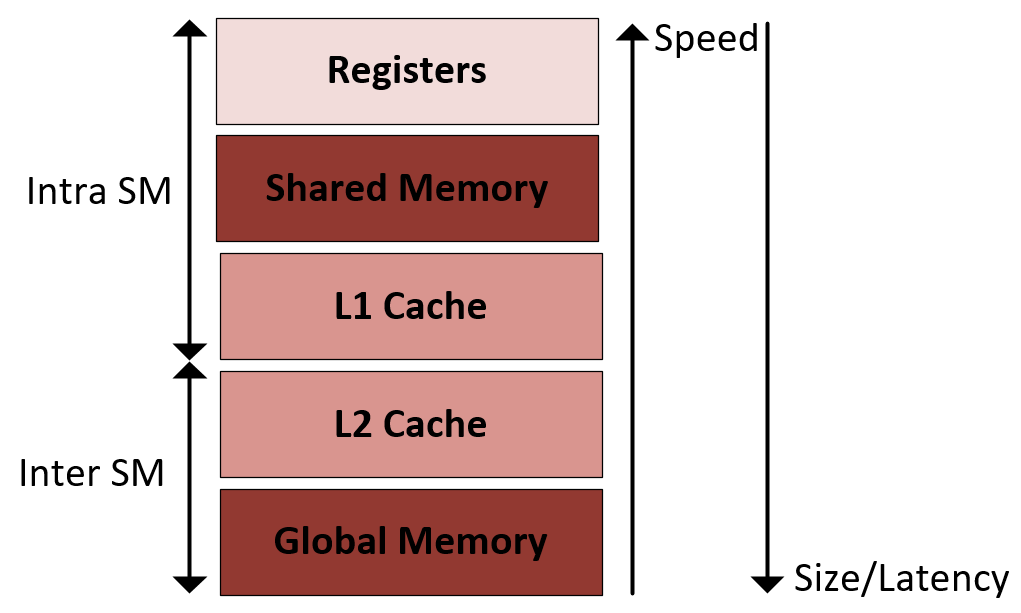
\includegraphics[width=0.6\textwidth]{figs/hw/hw-memory-schematic}}
	\caption{GPU memory schematic}
	\label{fig:hw-memory-schematic}
\end{figure}

\begin{figure}[H]
	\centering
	\fbox{
		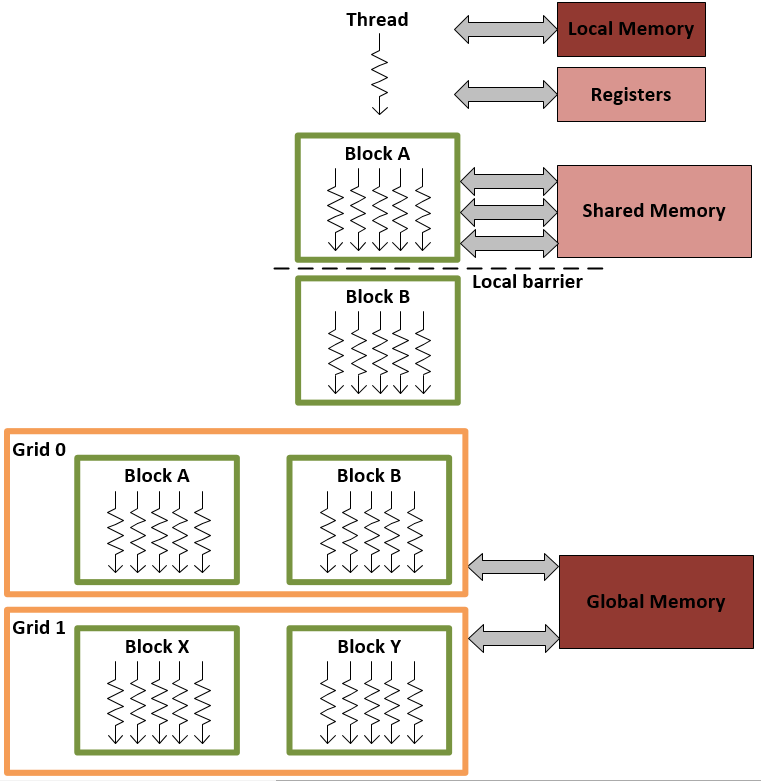
\includegraphics[width=1\textwidth]{figs/hw/hw-memory-model}}
	\caption{GPU memory access scopes}
	\label{fig:hw-memory-model}
\end{figure}

